\section{Technische Dokumentation}

\subsection{Einleitung}

Die generelle Zielsetzung sah die Erstellung eines Tools vor, das auf Grundlage von Benutzerpräferenzen personalisierte Reisevorschläge erstellt. Nutzer sollten in der Lage sein, Konten zu führen und ihre Reisen zu speichern.
Zusätzlich sollte – nach Möglichkeit – das Tool durch eine anschließende Datenanalyse, bzw. eine Datenvisualisierung erweitert werden.  

\subsection{Architekturübersicht}

\begin{figure}[h]
  \centering
  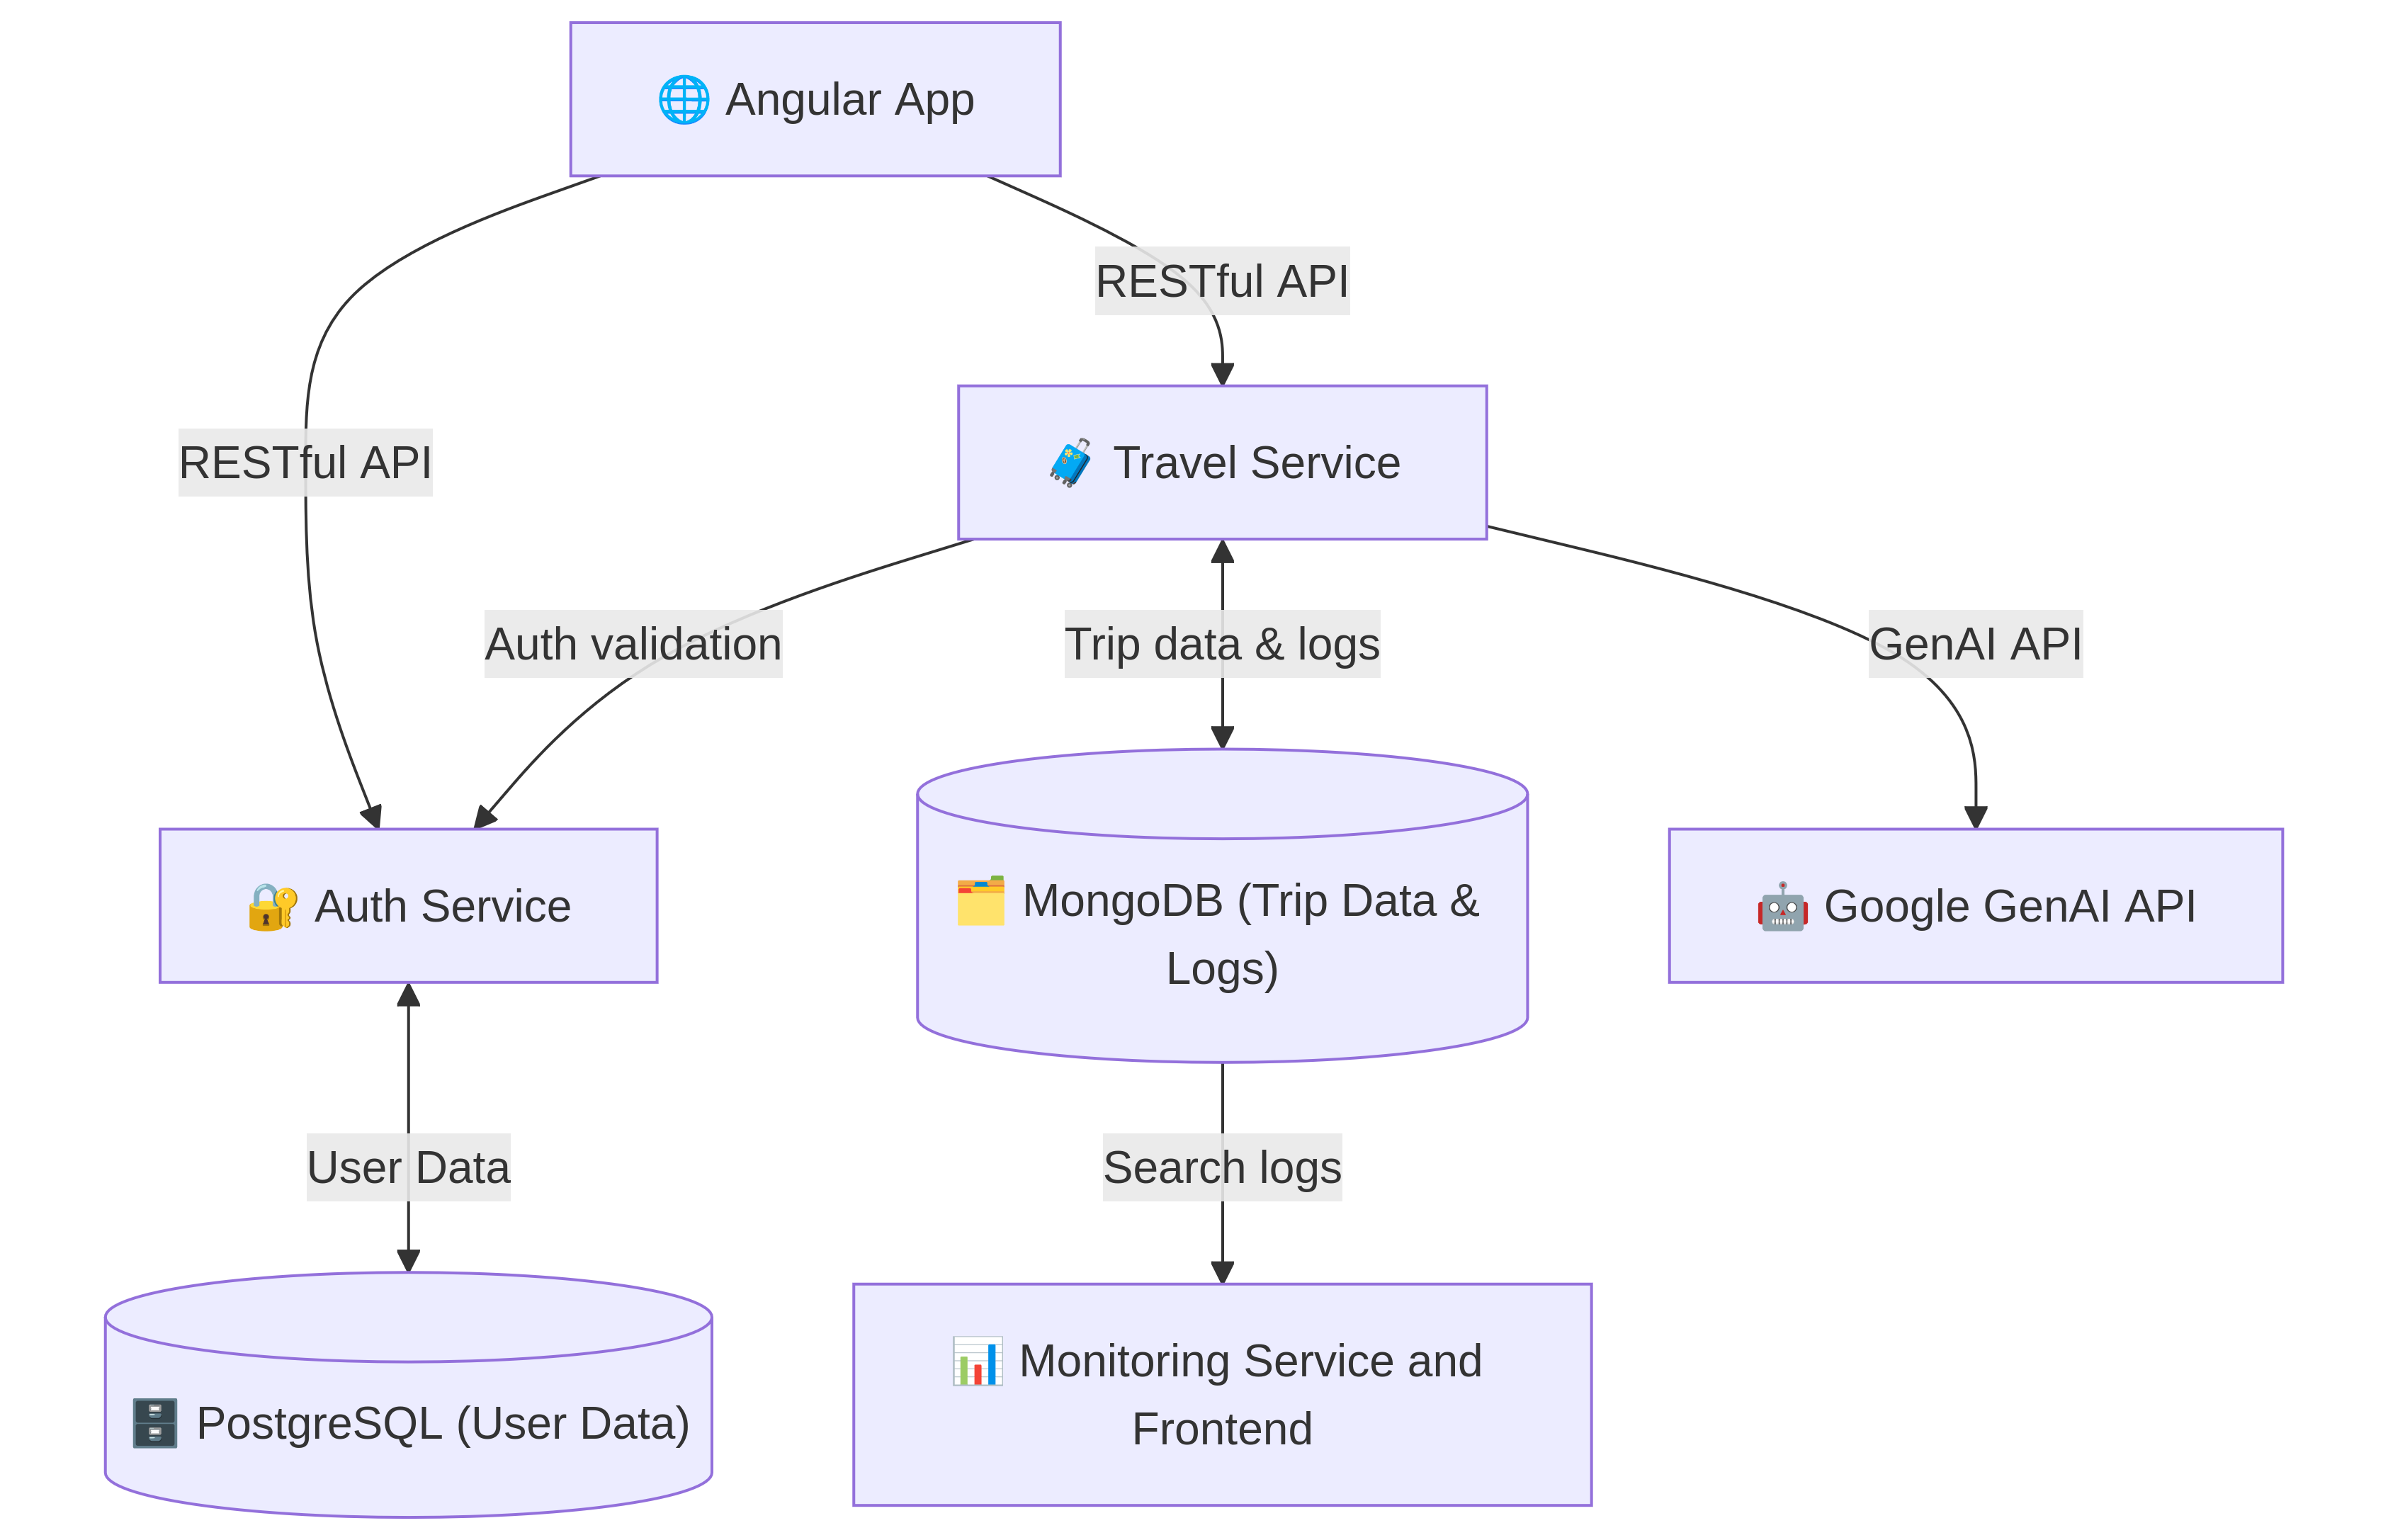
\includegraphics[width=0.8\textwidth]{images/architecture.png}
  \caption{Architekturübersicht des verteilten Systems}
\end{figure}

Die Abbildung zeigt die Architektur des entwickelten Systems. Man sieht hier ganz oben das Frontend, das mit Angular umgesetzt wurde. Es kommuniziert über REST-APIs mit zwei Microservices. Diese Microservices sind der Authentifizierungsservice und der Travel-Planner-Service. Es werden Datenbanken benutzt, um Nutzerdaten, Reisedaten und Log-Daten zu speichern. Für die Logik wird eine externe API von Google GenAI für die Generierung von Reiseempfehlungen eingebunden.

Das Backend ist in zwei separate Microservices unterteilt:
\begin{itemize}
  \item \textbf{auth\_service}: übernimmt die Authentifizierung und Verwaltung von Nutzerkonten und Präferenzen
  \item \textbf{travel\_service}: verarbeitet Nutzeranfragen, verwaltet geplante Reisen und generiert personalisierte Empfehlungen
\end{itemize}

Abschließend wurden sämtliche Anwendungen containerisiert und über ein Kubernetes-Cluster orchestriert. Dies ermöglicht eine standardisierte, skalierbare und portable Bereitstellung der Anwendung.


\subsection{Frontend}

Wie in der Vorlesung vorgestellt, wird hier auch Angular als Framework für die Frontend-Entwicklung eingesetzt. Angular basiert auf einem MVC-Pattern, das eine klare Trennung von Logik, Daten und Darstellung ermöglicht.
Konkret bei Angular werden Models durch die Typescript-Interfaces und Angular Services realisiert. Die Views werden durch HTML-Templates und CSS-Stile definiert, während die Controller-Logik in TypeScript-Klassen implementiert wird. Diese Struktur lässt den Code sehr gut modularisieren.

Angular eignet sich in diesem Fall besonders gut, da es eine reaktive Programmierung unterstützt und somit eine dynamische Benutzeroberfläche ermöglicht. Die Kommunikation mit den Backend-Microservices erfolgt über REST-APIs, die JSON-Daten austauschen, was ein guter Standard ist und ohne Probleme in verteilten Systemen funktioniert.

\subsubsection{Komponenten}
Die Angular-Anwendung besteht aus mehreren Komponenten, die jeweils für bestimmte Funktionalitäten zuständig sind. Die wichtigsten Komponenten sind:

\begin{itemize}
  \item \textbf{LoginComponent}: Ermöglicht die Anmeldung von Nutzern
  \item \textbf{RegisterComponent}: Ermöglicht die Registrierung neuer Nutzer
  \item \textbf{HomeComponent}: Zeigt die Startseite mit gespeicherten Reisen an
  \item \textbf{TripComponent}: Zeigt Details zu geplanten Reisen an.
  \item \textbf{RecommendationsComponent}: Ermöglicht die Eingabe von Reisepräferenzen und zeigt generierte Empfehlungen an. Später lässt sich hier auch eine Reise speichern.
\end{itemize}

Jeder dieser Komponenten hat eine eigene HTML-Template-Datei, die das Layout definiert, sowie eine TypeScript-Datei, die die Logik und Interaktion mit den Backend-Services implementiert. Die Kommunikation mit den Microservices erfolgt über Angular Services, die HTTP-Anfragen an die REST-APIs senden und die Antworten verarbeiten.

\subsubsection{Angular Services}

Die Angular-Anwendung nutzt Services, um die Kommunikation mit den Backend-Microservices zu abstrahieren. Diese Services kapseln die HTTP-Anfragen und ermöglichen eine einfache Wiederverwendbarkeit der Logik in verschiedenen Komponenten.
Hier gibt es drei zentrale Services:

\begin{itemize}
  \item \textbf{AuthService}: Verwaltet die Authentifizierungvon Nutzern, indem er mit dem Authentifizierungsservice kommuniziert. Er stellt Methoden zum Anmelden, Registrieren und Abrufen von Benutzerdaten bereit.
  \item \textbf{SuggestionService}: Kommuniziert mit dem Travel-Planner-Microservice, um Reiseempfehlungen zu generieren und geplante Reisen zu verwalten.
  \item \textbf{TripService}: Ist für das Abrufen und Speichern von Reisedaten zuständig.
\end{itemize}

Außerdem ist ein Interceptor implementiert, der alle HTTP-Anfragen abfängt und den JWT-Token für die Authentifizierung an die Header anhängt. Dies ermöglicht eine sichere Kommunikation mit den Microservices, ohne dass der Token manuell in jeder Anfrage hinzugefügt werden muss.


\subsection{Microservice-Architektur}

Das Backend wurde mithilfe von FastAPI in zwei Microservices umgesetzt. Die Architektur folgt dem Prinzip der Modularisierung und entspricht dem in der Vorlesung behandelten Aufbau verteilter Systeme.

\subsubsection{REST-APIs}

Beide Microservices bieten REST-APIs an. Es wurde bewusst auf gRPC und Event-basierte Kommunikation verzichtet, um die Komplexität zu reduzieren und eine einfache Integration mit dem Frontend zu ermöglichen. REST-APIs haben sich als Standard bewährt und sind sehr gut integrierbar, insbesondere in Kombination mit Angular. Die APIs sind so gestaltet, dass sie JSON-Daten austauschen, was eine einfache Handhabung und Verarbeitung der Daten ermöglicht.

Schnittstellen mit gRPC hätte eventuell Vorteile in Bezug auf Performance und Typensicherheit bieten können, vor allem wenn wir mit vielen verschiedenen abhängigen Services arbeiten. gRPC ist jedoch nicht direkt in Angular integriert und würde die Komplexität erhöhen.

Event-basierte Kommunikation hätte eine asynchrone Verarbeitung ermöglicht, was in diesem Fall jedoch gar nicht notwendig war.

\subsubsection{Containerisierung und Orchestrierung}

Beide Microservices wurden containerisiert und in einem Docker-Setup betrieben. Aufbau, Build und Deployment der Container orientieren sich an den in der Vorlesung vermittelten Grundlagen.

Die containerisierten Microservices wurden in einem Kubernetes-Cluster orchestriert. Damit wurde ein praxisnaher Anwendungsfall der in der Vorlesung behandelten Themen zu Skalierung und Verwaltung verteilter Systeme umgesetzt.

\subsubsection{Authentifizierungs-Microservice}

Der entwickelte Authentifizierungs-Microservice dient der Verwaltung von Benutzerkonten sowie der Authentifizierung registrierter Benutzer. Ziel ist es, auf Grundlage einer sicheren und überprüfbaren Identität weitere Microservices – insbesondere den Travel-Planner-Service – vor unberechtigtem Zugriff zu schützen. Die Implementierung erfolgt auf Basis des Python-Webframeworks FastAPI, das sich insbesondere durch seine hohe Performance, asynchrone Unterstützung und einfache OpenAPI- Integration (Swagger UI) auszeichnet. Letztere ermöglicht die einfache Interaktion mit den bereitgestellten REST-Endpunkten.

Zur Datenvalidierung kommt Pydantic v2 zum Einsatz. Diese Bibliothek erlaubt eine deklarative Modellierung und Validierung von Datenstrukturen auf Basis von Python-Typannotationen. Durch Pydantic wird sichergestellt, dass Nutzerdaten wie E-Mail-Adresse, Passwort und vollständiger Name beim Eintreffen überprüft und ggf. abgewiesen werden, bevor sie weiterverarbeitet werden. Dies stellt eine zentrale Maßnahme zur Stärkung der Systemsicherheit dar.

Die Speicherung von Passwörtern erfolgt unter Verwendung des bcrypt-Algorithmus, einem bewährten Verfahren zur sicheren und einwegigen Hashing-Verarbeitung sensibler Daten. Bcrypt schützt insbesondere gegen Brute-Force-Angriffe und Rainbow-Table-Attacken.

Für die Authentifizierung wurde ein JWT-basiertes (JSON Web Token) Verfahren implementiert. Beim erfolgreichen Login wird ein signierter Token generiert, der die Identität des Nutzers in Form eines sogenannten Claims (z.B. die E-Mail-Adresse) enthält. Dieser Token kann anschließend von anderen Microservices – z.B. dem Travel Planner – zur Authentifizierung des Nutzers verwendet werden, ohne dass das Passwort erneut übertragen werden muss. Damit wird das Prinzip der stateless Authentication umgesetzt, was insbesondere in verteilten Systemarchitekturen von Vorteil ist.

Die Benutzerinformationen werden in einer PostgreSQL-Datenbank persistiert. PostgreSQL wurde aufgrund seiner Zuverlässigkeit, Transaktionssicherheit und guten Integration in Python-Projekte ausgewählt.

Die gesamte Systemarchitektur orientiert sich am HATEOAS-Prinzip (Hypermedia as the Engine of Application State). Dadurch werden dem Client über die API nicht nur Daten, sondern auch Informationen über mögliche nächste Schritte zur Verfügung gestellt. Dies trägt zu einer entkoppelten, wartbaren Struktur bei und erleichtert die Integration mehrerer Microservices.

\subsubsection{Travel-Microservice}

Der Travel-Planner-Microservice ist für die Verarbeitung von Nutzeranfragen und die Generierung personalisierter Reiseempfehlungen zuständig. Er kommuniziert mit dem Authentifizierungs-Microservice, um sicherzustellen, dass nur authentifizierte Nutzer auf die Funktionen eines Profis zugreifen können.

Die Implementierung erfolgt ebenfalls mit FastAPI, um eine konsistente und performante API zu gewährleisten. Der Microservice nutzt die Google GenAI API, um auf Basis der Nutzerpräferenzen personalisierte Reiseempfehlungen zu generieren. Diese Empfehlungen werden in einem strukturierten Format zurückgegeben, das sowohl Reisedetails als auch allgemeine Tipps enthält.

Es gibt zusätzlich zu den Endpunkten für die Generierung von Reiseempfehlungen auch Endpunkte zum Speichern und Abrufen von Reisen. Diese Funktionalität ermöglicht es Nutzern, ihre geplanten Reisen zu speichern und später wieder abzurufen. Die gespeicherten Reisen werden in einer MongoDB-Datenbank persistiert, die sich gut für unstrukturierte Daten eignet und eine flexible Schema-Definition ermöglicht.

Auch werden hier Log-Daten erfasst, die für die spätere Analyse und Visualisierung der Nutzung des Systems verwendet werden können. Diese Log-Daten werden in einer separaten MongoDB-Datenbank gespeichert und enthalten Informationen über häufige Suchanfragen, beliebte Reiseziele und andere relevante Metriken.

\subsection{Kompromisse und Abweichungen}

Im Rahmen der Entwicklung wurden einige Kompromisse und Abweichungen von den ursprünglich geplanten Zielen vorgenommen:

\begin{itemize}
  \item Die Implementierung der Logik für die Generierung von Reiseempfehlungen wurde aufgrund des Umfangs und der Komplexität auf die Nutzung der Google GenAI API beschränkt. Dadurch konnte die Funktionalität schneller bereitgestellt werden, allerdings wurde die Möglichkeit einer eigenen Implementierung komplexer Logik aufgegeben.
  \item Die Authentifizierung wurde hier selbst implementiert und birgt sicherlich einige Sicherheitsrisiken, die bei einem professionellen Deployment berücksichtigt werden müssten. Idealerweise sollte hier ein bewährter ID-Provider wie Google verwendet werden, damit die Sicherheit und Skalierbarkeit gewährleistet ist. In diesem Projekt wurde jedoch bewusst auf eine eigene Implementierung gesetzt, um die Funktionsweise besser zu verstehen und den Aufwand zu verringern.
  \item Das Monitoring und die Analyse der Log-Daten ist sehr grundlegend umgesetzt. Es ist ersichtlich, dass hier nocht viel Potenzial für Verbesserungen besteht. Dieser Service soll eine bloße Demonstration davon sein, dass es möglich ist, Log-Daten zu sammeln und auszuwerten. Es gibt keine Authentifizierung für den Zugriff auf die Log-Daten, was in einer produktiven Umgebung ein Sicherheitsrisiko darstellen würde. Die Daten werden nur sehr grundlegend dargestellt. 
\end{itemize}
